% Báo cáo xử lý phản hồi của các thầy (buổi họp 13/11/2026).
% Biên dịch bằng XeLaTeX: bash build_report.sh  (bảng lớn do make_report_tables.py tạo trong report_tables/)
\documentclass[11pt,a4paper]{article}

\usepackage{fontspec}
\setmainfont{Times New Roman}
\setmonofont[Scale=0.88]{Courier New}
\usepackage[vietnamese]{babel}
\usepackage[a4paper,margin=2.5cm]{geometry}
\usepackage{amsmath,amssymb}
\usepackage{booktabs,array,multirow,longtable,tabularx}
\usepackage{graphicx}
\usepackage{enumitem}
\usepackage{caption}
\usepackage{float}
\usepackage[colorlinks=true,linkcolor=black,urlcolor=blue!50!black]{hyperref}


\setlength{\parskip}{4pt}
\emergencystretch=3em
\setlist{itemsep=2pt,topsep=3pt}
\captionsetup{font=small,labelfont=bf}
\renewcommand{\arraystretch}{1.15}
\setlength{\LTpre}{6pt}\setlength{\LTpost}{6pt}
\providecommand{\tightlist}{\setlength{\itemsep}{0pt}\setlength{\parskip}{0pt}}
\graphicspath{{latex/figures/}}
\newcommand{\ours}{\textbf{STRIDE}}

\title{\textbf{Báo cáo xử lý phản hồi của các thầy}\\[2pt]\large Buổi họp ngày 13/11/2026}
\author{Nhóm NCKH UIT}
\date{Cập nhật ngày 19 tháng 11 năm 2026}

\begin{document}
\maketitle

Báo cáo trình bày những gì nhóm đã làm theo phản hồi của các thầy, để các thầy xem xét trước khi nhóm viết lại bài. Kết quả mang tính thăm dò (exploratory), trừ các kết quả ghi là ``xác nhận'': chúng được chạy đúng một lần trên tập topology kiểm tra chưa dùng, với hệ số và tiêu chí ghi trước. Các ngưỡng đạt/không đạt do nhóm tự đặt, không phải chuẩn bên ngoài.

Phương pháp có tên STRIDE (Skeleton-Tolerant Re-selecting Intervals for Dynamic Effects), kèm bước hiệu chỉnh độ rộng ở mức topology. Các tài liệu đã đóng băng trước đó gọi nó là SRCI.

\section{Điều kiện đủ để coverage đúng}

Trước đây hệ số nới độ rộng là một phân vị gộp ở mức cặp trên khoảng 20 topology. Nó nhắm tới độ phủ trung bình 0,95 nhưng không bảo đảm gì cho từng topology: kiểm tra cho thấy nó xấp xỉ trung vị của điểm theo topology, tức khoảng một nửa số topology vẫn trượt nhiều hơn mức mong muốn.

Các khái niệm dùng trong phần này:

\begin{itemize}
\tightlist
\item
  Cặp non-null: cặp (biến nguồn, biến đích) có hiệu ứng thật khác 0 trong mô hình sinh dữ liệu; coverage chỉ đo trên các cặp này. Cặp bị trượt (missed) khi giá trị thật nằm ngoài khoảng tin cậy.
\item
  Điểm của topology (unit score): hệ số nới nhỏ nhất để không quá $\beta=10\%$ số cặp non-null bị trượt, lấy giá trị lớn nhất trên hai mức hỏng. Topology ``đạt ngưỡng'' (hit) nếu điểm không vượt hệ số đang dùng.
\item
  Tỉ lệ topology đạt ngưỡng (topology hit rate): phần trăm topology kiểm tra đạt ngưỡng; đây là đại lượng mà bảo đảm nhắm tới, mục tiêu 0,90.
\item
  Hệ số hiệu chỉnh $c$: xếp $N$ điểm của $N$ topology hiệu chỉnh theo thứ tự tăng dần rồi lấy điểm ở hạng $k_0$ (order statistic). Có hai cách chọn $k_0$:

  \begin{itemize}
  \tightlist
  \item
    Phiên bản biên (marginal): $k_0=\lceil (N+1)(1-\delta)\rceil$, $\delta=0{,}10$. Nếu topology hiệu chỉnh và kiểm tra hoán vị được thì xác suất một topology mới đạt ngưỡng ít nhất là $k_0/(N+1)$. Đây là bảo đảm trung bình trên mọi cách rút tập hiệu chỉnh; với một tập cụ thể, tỉ lệ đạt thật có thể thấp hơn 0,90 do may rủi của mẫu.
  \item
    Phiên bản PAC (probably approximately correct): $k_0$ là hạng nhỏ nhất sao cho phân phối $\mathrm{Beta}(k_0,\,N+1-k_0)$ tại 0,90 không quá 0,05. Khi đó, với độ tin cậy 0,95 theo mẫu hiệu chỉnh, ít nhất 90\% topology mới đạt ngưỡng. Cần $N\geq 59$. Với $N=550$, bản biên lấy hạng 496, bản PAC lấy hạng 507, nên khoảng rộng hơn khoảng 5\%.
  \end{itemize}
\end{itemize}

Điều kiện hoán vị được bảo đảm bằng cách xây dựng tập topology. Nhóm sinh 1.200 topology độc lập từ cùng một bộ sinh và chia ngẫu nhiên thành ba phần: thiết kế (100), hiệu chỉnh (550) và kiểm tra (550). Một tập thí điểm gồm 360 topology (60/150/150) được dùng để chọn quy tắc và viết mã; phần kiểm tra của tập này chỉ được mở một lần, để chấm cờ độ tin cậy ở lag 1. Ở các tập cũ, tập hiệu chỉnh và tập kiểm chứng là các tập cố định nên không có cơ sở hoán vị như vậy.

Mệnh đề chỉ áp dụng cho topology mới cùng họ bộ sinh, trong kịch bản sạch, hỏng một loại và khai báo đúng; nó không nói gì về từng cặp riêng lẻ, dữ liệu thật, nhiễu đuôi dày hay khai báo sai. Bản phác thảo chứng minh do nhóm phản biện nội bộ soạn và chưa được người ngoài thẩm định.

Kết quả xác nhận đo trên 550 topology kiểm tra cho từng lag, với hệ số đóng băng và tiêu chí ghi trước.

Bảng dưới đây cho kết quả theo từng ô (cell), tức từng tổ hợp (lag, $T$, loại hỏng): lag 1 có 5 giá trị $T$ $\times$ 4 loại hỏng = 20 ô, lag 2 có 16 ô và lag 3 có 12 ô. Các cột là:

\begin{itemize}
\tightlist
\item
  Hệ số (biên): hệ số hiệu chỉnh $c$ của phiên bản biên. ``Từ chối'' nghĩa là bước hiệu chỉnh không tìm được hệ số hữu hạn nên phương pháp không đưa ra bảo đảm (abstain).
\item
  Tỉ lệ đạt: luật cũ, Biên và PAC: tỉ lệ topology đạt ngưỡng trên 550 topology kiểm tra khi dùng luật cũ, hệ số biên và hệ số PAC. Mục tiêu là 0,90.
\item
  Biên {[}CI 95\%{]}: khoảng tin cậy 95\% của tỉ lệ đạt ngưỡng ở phiên bản biên.
\item
  Chạm 0,90: ``có'' nếu cận trên của khoảng tin cậy đó không thấp hơn 0,90, tức kết quả phù hợp với mục tiêu.
\end{itemize}

{\small
\begin{longtable}{llllrrrc}
\caption{Tỉ lệ topology đạt ngưỡng theo từng ô (lag, $T$, loại hỏng), trên 550 topology kiểm tra. Mục tiêu là $0{,}90$.}\label{tab:guarantee}\\
\toprule
Lag & T & Loại hỏng & Hệ số (biên) & Luật cũ & Biên [CI 95\%] & PAC & Chạm 0,90 \\
\midrule
\endfirsthead
\toprule
Lag & T & Loại hỏng & Hệ số (biên) & Luật cũ & Biên [CI 95\%] & PAC & Chạm 0,90 \\
\midrule
\endhead
\bottomrule
\endfoot
\multirow{20}{*}{1} & \multirow{4}{*}{19} & Không hỏng & 3,888 & 0,869 & 0,922 [0,896; 0,943] & 0,935 & có \\
 &  & Thừa cạnh & 4,044 & 0,780 & 0,922 [0,896; 0,943] & 0,936 & có \\
 &  & Thiếu cạnh & 2,657 & 0,789 & 0,889 [0,860; 0,914] & 0,920 & có \\
 &  & Đảo cạnh & 4,443 & 0,767 & 0,886 [0,857; 0,912] & 0,907 & có \\
\cmidrule(l){2-8}
 & \multirow{4}{*}{30} & Không hỏng & 3,473 & 0,825 & 0,864 [0,832; 0,891] & 0,885 & không \\
 &  & Thừa cạnh & 3,514 & 0,775 & 0,871 [0,840; 0,898] & 0,895 & không \\
 &  & Thiếu cạnh & 3,119 & 0,775 & 0,875 [0,844; 0,901] & 0,909 & có \\
 &  & Đảo cạnh & 3,895 & 0,780 & 0,866 [0,835; 0,894] & 0,899 & không \\
\cmidrule(l){2-8}
 & \multirow{4}{*}{40} & Không hỏng & 3,598 & 0,858 & 0,902 [0,874; 0,925] & 0,925 & có \\
 &  & Thừa cạnh & 3,722 & 0,778 & 0,927 [0,902; 0,948] & 0,933 & có \\
 &  & Thiếu cạnh & 3,297 & 0,807 & 0,922 [0,896; 0,943] & 0,933 & có \\
 &  & Đảo cạnh & 3,957 & 0,791 & 0,905 [0,877; 0,928] & 0,936 & có \\
\cmidrule(l){2-8}
 & \multirow{4}{*}{80} & Không hỏng & 2,983 & 0,885 & 0,920 [0,894; 0,941] & 0,933 & có \\
 &  & Thừa cạnh & 3,04 & 0,820 & 0,920 [0,894; 0,941] & 0,936 & có \\
 &  & Thiếu cạnh & 2,836 & 0,831 & 0,913 [0,886; 0,935] & 0,944 & có \\
 &  & Đảo cạnh & 3,374 & 0,800 & 0,907 [0,879; 0,930] & 0,919 & có \\
\cmidrule(l){2-8}
 & \multirow{4}{*}{150} & Không hỏng & 2,59 & 0,818 & 0,876 [0,846; 0,903] & 0,900 & có \\
 &  & Thừa cạnh & 2,734 & 0,789 & 0,895 [0,866; 0,919] & 0,902 & có \\
 &  & Thiếu cạnh & 2,584 & 0,793 & 0,875 [0,844; 0,901] & 0,896 & có \\
 &  & Đảo cạnh & 3,003 & 0,771 & 0,888 [0,859; 0,913] & 0,908 & có \\
\midrule
\multirow{16}{*}{2} & \multirow{4}{*}{30} & Không hỏng & từ chối & 0,762 & --- & --- & --- \\
 &  & Thừa cạnh & từ chối & 0,671 & --- & --- & --- \\
 &  & Thiếu cạnh & từ chối & 0,438 & --- & --- & --- \\
 &  & Đảo cạnh & từ chối & 0,566 & --- & --- & --- \\
\cmidrule(l){2-8}
 & \multirow{4}{*}{40} & Không hỏng & 3,653 & 0,827 & 0,889 [0,860; 0,914] & 0,909 & có \\
 &  & Thừa cạnh & 3,664 & 0,782 & 0,891 [0,862; 0,916] & 0,916 & có \\
 &  & Thiếu cạnh & 3,118 & 0,782 & 0,904 [0,876; 0,927] & 0,916 & có \\
 &  & Đảo cạnh & 4,133 & 0,765 & 0,890 [0,860; 0,915] & 0,910 & có \\
\cmidrule(l){2-8}
 & \multirow{4}{*}{80} & Không hỏng & 2,79 & 0,847 & 0,900 [0,872; 0,924] & 0,916 & có \\
 &  & Thừa cạnh & 2,797 & 0,807 & 0,869 [0,838; 0,896] & 0,902 & không \\
 &  & Thiếu cạnh & 2,684 & 0,776 & 0,904 [0,876; 0,927] & 0,915 & có \\
 &  & Đảo cạnh & 3,093 & 0,790 & 0,868 [0,836; 0,895] & 0,893 & không \\
\cmidrule(l){2-8}
 & \multirow{4}{*}{150} & Không hỏng & 2,462 & 0,873 & 0,896 [0,868; 0,921] & 0,916 & có \\
 &  & Thừa cạnh & 2,543 & 0,816 & 0,891 [0,862; 0,916] & 0,922 & có \\
 &  & Thiếu cạnh & 2,514 & 0,798 & 0,927 [0,902; 0,948] & 0,938 & có \\
 &  & Đảo cạnh & 2,856 & 0,792 & 0,851 [0,818; 0,880] & 0,888 & không \\
\midrule
\multirow{12}{*}{3} & \multirow{4}{*}{40} & Không hỏng & từ chối & 0,585 & --- & --- & --- \\
 &  & Thừa cạnh & từ chối & 0,507 & --- & --- & --- \\
 &  & Thiếu cạnh & từ chối & 0,071 & --- & --- & --- \\
 &  & Đảo cạnh & từ chối & 0,531 & --- & --- & --- \\
\cmidrule(l){2-8}
 & \multirow{4}{*}{80} & Không hỏng & 2,87 & 0,845 & 0,887 [0,858; 0,912] & 0,904 & có \\
 &  & Thừa cạnh & 2,94 & 0,755 & 0,882 [0,852; 0,908] & 0,900 & có \\
 &  & Thiếu cạnh & 2,718 & 0,740 & 0,876 [0,846; 0,903] & 0,893 & có \\
 &  & Đảo cạnh & 3,18 & 0,778 & 0,879 [0,848; 0,905] & 0,886 & có \\
\cmidrule(l){2-8}
 & \multirow{4}{*}{150} & Không hỏng & 2,424 & 0,889 & 0,891 [0,862; 0,916] & 0,915 & có \\
 &  & Thừa cạnh & 2,544 & 0,835 & 0,895 [0,866; 0,919] & 0,918 & có \\
 &  & Thiếu cạnh & 2,461 & 0,804 & 0,911 [0,884; 0,933] & 0,935 & có \\
 &  & Đảo cạnh & 2,848 & 0,767 & 0,882 [0,852; 0,908] & 0,897 & có \\
\end{longtable}
}


Kết quả: 17/20 ô chạm 0,90 ở lag 1 (85\%), 9/12 ô có hệ số ở lag 2 (75\%) và 8/8 ô có hệ số ở lag 3. Tiêu chí ghi trước là ít nhất 80\% số ô có hệ số phải chạm 0,90, nên đạt ở lag 1 và lag 3, không đạt ở lag 2.

So với luật cũ, trên cùng các ô có hệ số hữu hạn, khoảng tin cậy rộng hơn $\times$1,18, $\times$1,14 và $\times$1,10 và interval score cao hơn 11\%, 6\% và 3\% (lần lượt ở lag 1, 2, 3, với hệ số biên). Phiên bản PAC rộng hơn khoảng 5\% so với phiên bản biên.

Ở lag 2, tiêu chí ghi trước không đạt (75\% so với 80\%), nên theo đặc tả nhóm rút tuyên bố bảo đảm ở ba ô: $T=80$ thừa cạnh, $T=80$ đảo cạnh và $T=150$ đảo cạnh (cận trên nhỏ nhất ở lag 2 vẫn là 0,880). Ở lag 2 với $T=30$ và lag 3 với $T=40$, phương pháp từ chối đưa ra bảo đảm (abstain) vì 9\% đến 92\% số lượt fit thất bại. Tại các ô này, luật cũ vẫn trả về khoảng tin cậy nhưng chỉ 7\% đến 76\% topology đạt ngưỡng (thấp nhất 7\% ở lag 3, $T=40$, thiếu cạnh); vì vậy hệ số mới còn cho biết khi nào không nên tin khoảng tin cậy. Ở các ô đạt, tỉ lệ đạt ngưỡng quanh 0,89--0,90, sát mục tiêu và không dư (sai số lấy mẫu của 550 topology khoảng $\pm$0,025). Toàn bộ kết quả dùng một bộ sinh, 14 nút, 21 cạnh và nhiễu Gaussian sạch.

\section{Hệ số 0,5}

Hệ số co (pre-shrink) $\kappa$ nhân vào nửa độ rộng của khoảng bootstrap trước bước hiệu chỉnh, nên khoảng cuối cùng là trung điểm $\pm$ $\kappa c\cdot(\text{nửa độ rộng})$. $\kappa=0{,}5$ làm nửa độ rộng co một nửa; $\kappa$ \textgreater{} 1 sẽ làm khoảng rộng ra. Hằng số này được thêm vì lưới hiệu chỉnh cũ chỉ cho phép nới (từ 1,0), trong khi ở $T$ nhỏ khoảng bootstrap vốn đã quá rộng. Không có cơ sở lý thuyết cho đúng giá trị 0,5. Nếu $\kappa$ áp dụng giống nhau ở hiệu chỉnh và kiểm tra thì khoảng cuối chỉ phụ thuộc tích $\kappa c$, nên bảo đảm ở phần trên không phụ thuộc giá trị này.

Nhóm kiểm độ nhạy bằng cách hiệu chỉnh theo quy tắc cũ trên tập hiệu chỉnh và đánh giá trên tập thiết kế. Quy tắc cũ chọn hệ số $c$ từ một lưới giá trị định sẵn, bắt đầu từ 1,0 (grid floor, tạm gọi là sàn lưới) và chỉ cho phép nới, không cho thu hẹp. Hệ số hiệu dụng (effective factor) là $\kappa\times c$, tức bội số thực sự nhân vào nửa độ rộng của khoảng bootstrap. Cột ``số ô chạm sàn lưới'' đếm số ô (trên 20) mà c được chọn đúng bằng 1,0, nghĩa là phép hiệu chỉnh muốn thu hẹp thêm nhưng lưới không cho.

\begin{table}[H]
\centering
\caption{Độ nhạy theo hệ số co $\kappa$ (hiệu chỉnh trên tập hiệu chỉnh, đánh giá trên tập thiết kế).}\label{tab:kappa}
{\small
\begin{tabular}{lrrrr}
\toprule
Hệ số co $\kappa$ & Hệ số hiệu dụng & Số ô chạm sàn lưới & Coverage & Interval score \\
\midrule
0,25 & 1,424 & 0/20 & 0,951 & 5,24 \\
0,5 & 1,435 & 0/20 & 0,952 & 5,26 \\
1,0 & 1,460 & 0/20 & 0,955 & 5,33 \\
2,0 & 2,000 & 20/20 & 0,988 & 6,55 \\
\bottomrule
\end{tabular}
}
\end{table}


Với $\kappa$ từ $0{,}25$ đến $1{,}0$, kết quả gần như trùng nhau và chênh lệch chủ yếu do làm tròn của lưới. Với $\kappa=2$, lưới chạm sàn nên khoảng tin cậy quá rộng. Như vậy giá trị 0,5 không quan trọng miễn là sàn của lưới không bị chạm, và nhóm đề xuất bỏ hằng số này, dùng hệ số là thống kê hạng chính xác (không qua lưới) như ở phần Điều kiện đủ để coverage đúng.

\section{T nhỏ nhất và mức hỏng mà phương pháp còn chạy được}

Trên tập 1.200 topology (phần Điều kiện đủ), hệ số bảo đảm hữu hạn từ $T=19$ ở lag 1, từ $T=40$ ở lag 2 và từ $T=80$ ở lag 3. Dưới các ngưỡng này (lag 2 với $T=30$, lag 3 với $T=40$), tỉ lệ fit thất bại nằm trong khoảng 9\% đến 92\% và phương pháp từ chối đưa ra đảm bảo. Như vậy $T$ tối thiểu tăng theo số lag, phù hợp với bản đồ thăm dò đã có từ trước (19, 40 và 80 cho lag 1, 2 và 4).

Phần quét theo mức hỏng chỉ được chạy ở lag 1, trên 60 topology thiết kế của tập thí điểm ($T$ $\in$ \{19, 30, 40, 80, 150\}, mức hỏng từ 0,1 đến 0,8, ba loại hỏng, 14 nút và 21 cạnh). Quy tắc ghi trước: một ô được coi là dùng được nếu fit thành công ở ít nhất 95\% số lượt và coverage của các cặp non-null tại hệ số hiệu chỉnh đạt ít nhất 0,90. Với thiếu cạnh, phương pháp dùng được ở mọi $T$ đã thử, kể cả $T=19$ ở mức hỏng 0,8. Với thừa cạnh và đảo cạnh, phương pháp dùng được từ $T=30$ ở mọi mức đến 0,8; ở $T=19$, thừa cạnh thất bại từ mức 0,7 (tỉ lệ fit thành công 0,92 rồi 0,87) và đảo cạnh thất bại từ mức 0,5 (tỉ lệ thành công từ 0,92 xuống 0,88).

Kết quả quét có các hạn chế sau. ``Thành công'' chỉ nghĩa là bước fit hoàn tất; coverage chỉ tính trên các lần fit thành công; interval score chưa so với oracle; coverage cao (0,96 đến 0,99) là hệ quả của hệ số thận trọng ở mức topology. Đơn vị có số cạnh đảo bằng 0 ở mức hỏng thấp được xếp vào ô không hỏng và loại khỏi tỉ lệ thành công. Dữ liệu từ một nhánh phát triển khác (khai báo sai mức hỏng) cho thấy khi khai báo gấp đôi số cạnh thiếu ở mức 50\%, chỉ 5 đến 11 trong 60 lượt chạy được; nhóm tái lập được một phần và chưa đưa vào bài.

\section{Sơ đồ phương pháp}

\begin{figure}[H]
\centering
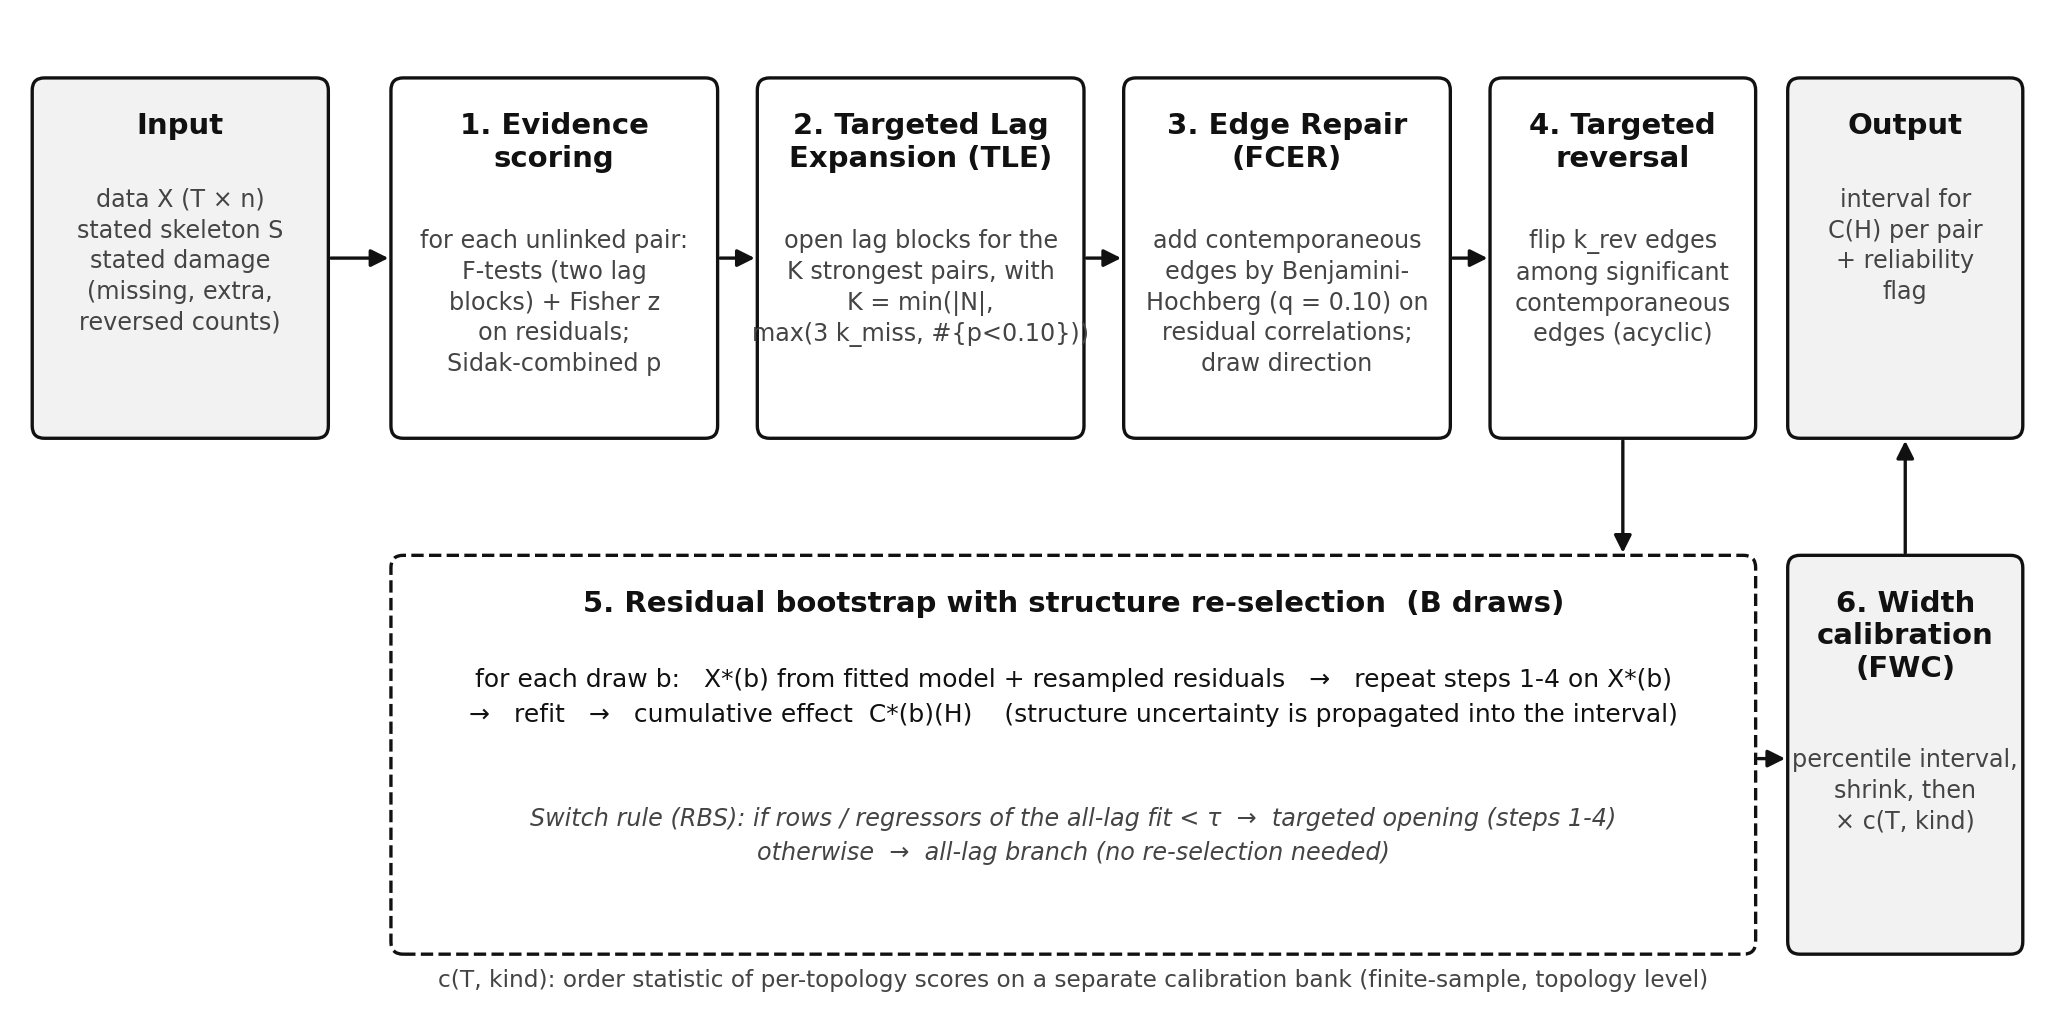
\includegraphics[width=\linewidth]{architecture_srci.png}
\caption{Sơ đồ phương pháp \ours{} (bản nháp, sẽ được chỉnh lại).}\label{fig:architecture}
\end{figure}

\section{Mô phỏng}

Nhóm đã viết bộ sinh tập topology có tham số (số topology, kích thước từng phần) và tạo hai tập mới gồm 360 và 1.200 topology, so với 40 topology trước đây. Các thực nghiệm đã chạy ở lag 1, 2 và 3 (phần Điều kiện đủ).

Để kiểm tra khi nhiễu không còn là Gaussian, nhóm giữ nguyên hệ số đóng băng và chạy lại trên các topology kiểm tra ở lag 1 với nhiễu động học Student-t bốn bậc tự do hoặc Laplace, phương sai bằng 1. Đây là các kịch bản vi phạm giả định Gaussian sạch và không nằm trong phạm vi bảo đảm.

\begin{table}[H]
\centering
\caption{Tỉ lệ topology đạt ngưỡng khi nhiễu động học không phải Gaussian (lag 1, hệ số Gaussian đóng băng).}\label{tab:noise}
{\small
\begin{tabular}{lrrr}
\toprule
Nhiễu & Tỉ lệ topology đạt ngưỡng: luật cũ / biên / PAC & Số ô chạm 0,90 & Độ rộng trung bình (biên) \\
\midrule
Gaussian (xác nhận) & 0,805 / 0,897 / 0,918 & 17/20 & 4,86 \\
Student-t(4) & 0,824 / 0,909 / 0,927 & 18/20 & 5,25 \\
Laplace & 0,812 / 0,901 / 0,921 & 17/20 & 6,29 \\
\bottomrule
\end{tabular}
}
\end{table}


Hệ số hiệu chỉnh trên Gaussian vẫn giữ tỉ lệ topology đạt ngưỡng ở mức 0,90 khi nhiễu động học đổi dạng, với khoảng tin cậy rộng hơn đôi chút (Laplace rộng hơn 29\%).

Kết quả khác hẳn khi thêm sai số đo, tức nhiễu cộng thêm vào dữ liệu quan sát với phương sai bằng 10\% hoặc 30\% phương sai của mỗi cột.

\begin{table}[H]
\centering
\caption{Tỉ lệ topology đạt ngưỡng khi dữ liệu có sai số đo (lag 1, hệ số Gaussian đóng băng).}\label{tab:me}
{\small
\begin{tabular}{lrrr}
\toprule
Sai số đo & Tỉ lệ đạt ngưỡng: luật cũ / biên / PAC & Dải giữa các ô (biên) & Coverage theo cặp (biên) \\
\midrule
Không & 0,805 / 0,897 / 0,918 & 0,86 đến 0,93 & 0,971 \\
10\% & 0,642 / 0,776 / 0,810 & 0,53 đến 0,93 & 0,948 \\
30\% & 0,363 / 0,501 / 0,544 & 0,03 đến 0,88 & 0,878 \\
\bottomrule
\end{tabular}
}
\end{table}


Bảo đảm không chịu được sai số đo, và tình hình xấu hơn khi $T$ lớn (với nhiễu 10\%, $T=150$ chỉ còn 0,53 đến 0,59), vì sai lệch do sai số đo không giảm khi có thêm dữ liệu. Kết quả này nhất quán với các thử nghiệm sơ bộ của một nhóm khác, trong đó coverage giảm xuống 0,66 đến 0,75. Đây là một hạn chế thật của phương pháp và bài cần nêu rõ. Hướng khắc phục (chẳng hạn ước lượng tỉ lệ nhiễu đo rồi nới khoảng, như nhánh adapt của kho mã gốc) chưa được đánh giá đầy đủ nên chưa đưa vào. Nhóm mong nhận ý kiến của các thầy về việc có nên thêm một tập topology với số nút khác 14 hay không.

\section{Tài liệu từ 2021 trở đi}

Nhóm đã kiểm chứng 79 mục (trong đó 69 mục từ 2021 trở đi), phân bố theo chủ đề như sau: conformal (17), IRF và SVAR (18), suy luận sau khi chọn mô hình hoặc khi đồ thị sai (10), học cấu trúc chuỗi thời gian (10), FDR (9), interval score (5), VAR trên dữ liệu Việt Nam (7) và sai số đo (3). Hai chủ đề còn mỏng là sai số đo trong mô hình nhân quả chuỗi thời gian và các nghiên cứu về Việt Nam. Việc kiểm chứng chủ yếu dựa trên Crossref; nhóm chưa đọc từng bài. Danh mục nằm ở \texttt{docs/latex/references\_2021.bib} và đã được nối vào bản thảo.

\section{Dữ liệu thực tế}

Panel gồm 14 biến: 3 biến vĩ mô và 4 biến cổ phiếu là dữ liệu thật, còn 7 biến ngân hàng là dữ liệu mô phỏng hiệu chỉnh, không phải số liệu thật; bài sẽ khai báo rõ điều này.

Trên panel hiện có (14 biến, 19 quý, skeleton 21 cạnh, hệ số mới, 5 hạt giống bootstrap, 3 mức khai báo), khoảng tin cậy của cả 10 cặp được chọn trước, ở mọi mức khai báo và mọi hạt giống, đều chứa 0. Các cặp giữa hai biến quan sát được (lãi suất chính sách tới lợi suất cổ phiếu, tới GDP và tới CPI; CPI tới khối lượng giao dịch) là dữ liệu thật; các cặp có biến ngân hàng chỉ mang tính minh họa. Khoảng tin cậy rộng ra khi khai báo nhiều cạnh thiếu hơn: ví dụ với cặp lãi suất chính sách tới lợi suất cổ phiếu, độ rộng là 0,92 khi không hỏng, 4,4 khi thiếu 20\% và 7,3 khi thiếu 50\%. Nói cách khác, 19 quý quá ngắn để xác định dấu của bất kỳ hiệu ứng nào trong các cặp đã chọn; phương pháp phản ánh đúng mức bất định đó thay vì tạo ra một kết quả có ý nghĩa kinh tế.

Để biết phương pháp hoạt động ra sao trong đúng vùng của panel, nhóm fit một mô hình động lên panel, coi nó là ground truth, sinh 400 chuỗi với $T=19$ và $n=14$, rồi làm hỏng skeleton ở ba mức (không hỏng, thiếu 20\% và thiếu 50\%).

\begin{table}[H]
\centering
\caption{Mô phỏng theo panel ($T=19$, $n=14$, 400 chuỗi) với hai phương pháp.}\label{tab:panel}
{\small
\begin{tabular}{llp{2.5cm}p{3.2cm}rr}
\toprule
Khai báo & Phương pháp & Coverage theo cặp non-null & Tỉ lệ lần sinh có $\leq$10\% cặp trượt & Độ rộng trung vị & Fit thành công \\
\midrule
Không hỏng & RB plug-in & 0,904 & 0,620 & 1,87 & 400/400 \\
Không hỏng & STRIDE & 0,990 & 0,990 & 3,64 & 400/400 \\
Thiếu 20\% & RB plug-in & 0,663 & 0,000 & 1,70 & 400/400 \\
Thiếu 20\% & STRIDE & 0,981 & 0,959 & 5,09 & 390/400 \\
Thiếu 50\% & RB plug-in & 0,291 & 0,000 & 1,45 & 400/400 \\
Thiếu 50\% & STRIDE & 0,993 & 0,978 & 13,94 & 359/400 \\
\bottomrule
\end{tabular}
}
\end{table}


``RB plug-in'' là phương pháp đối chứng: residual bootstrap (RB) cắm thẳng (plug-in) skeleton khai báo vào mô hình như thể nó đúng. Nó nhận cùng skeleton đã bị làm hỏng như STRIDE nhưng không nghi ngờ, không sửa cấu trúc và không dùng mức hỏng. STRIDE thì ngược lại: coi skeleton là giả thuyết có thể sai, kiểm tra và sửa nó trước khi dựng khoảng tin cậy. STRIDE giữ coverage ở mức 0,98 đến 0,99 trong khi RB giảm xuống 0,29 khi thiếu 50\% cạnh. Tuy nhiên, khi thiếu cạnh, một số lần sinh cho khoảng rộng đột biến (độ rộng trung bình lên tới vài trăm đến vài nghìn, trong khi trung vị chỉ từ 5 đến 14) và 10\% lần fit thất bại ở mức thiếu 50\%. Với $T=19$ và 11 cạnh thiếu, bài toán gần như vô định, và các thầy cần lưu ý điều này khi đọc phần ứng dụng. Kết quả dựa trên một ground truth duy nhất nên không phải bảo đảm theo topology, và panel gốc có 7 biến là mô phỏng.

\section{So sánh với các phương pháp tham chiếu ở cùng mức đảm bảo}

Mỗi phương pháp được hiệu chỉnh bằng cùng một quy tắc (thống kê hạng theo topology, $\beta=10\%$, $\delta=10\%$) trên cùng 150 topology hiệu chỉnh, rồi chạy một lần trên 200 topology kiểm tra (lag 1, $T=40$ và 150, bốn loại hỏng). Khi đó các phương pháp đạt cùng mức đảm bảo (tỉ lệ topology đạt ngưỡng quanh 0,90) và có thể so sánh bằng độ rộng và interval score.

Interval score trung bình (IS, càng thấp càng tốt) theo từng ô ($T$, loại hỏng) ở lag 1; in đậm là giá trị thấp nhất trong số các phương pháp đạt mức đảm bảo, dấu \(\dagger\) là phương pháp không đạt mức đảm bảo ở ô đó (cận trên của khoảng tin cậy 95\% của tỉ lệ topology đạt ngưỡng thấp hơn 0,90), nên không được xét để xếp hạng thấp nhất.

\begin{table}[H]
\centering
\caption{Interval score trung bình ở lag 1 (càng thấp càng tốt). In đậm là giá trị thấp nhất trong các phương pháp đạt mức đảm bảo; $^{\dagger}$ là phương pháp không đạt mức đảm bảo ở ô đó.}\label{tab:cmp-is}
{\small
\begin{tabular}{llrrrrrr}
\toprule
T & Loại hỏng & STRIDE & BVAR-Minnesota & PSel-Union & PSel & Full VAR & TLP \\
\midrule
\multirow{4}{*}{40} & Không hỏng & 4,15 & \textbf{3,83} & 5,10 & 5,24 & 4,67 & 4,46 \\
 & Thừa cạnh & 4,39 & \textbf{4,11} & 5,34 & 5,42 & 4,78 & 4,58 \\
 & Thiếu cạnh & \textbf{4,69} & 6,13 & 5,19 & 5,99 & 5,08 & 5,34 \\
 & Đảo cạnh & \textbf{4,66} & 4,94 & 5,59 & 5,81 & 5,26 & 4,95 \\
\midrule
\multirow{4}{*}{150} & Không hỏng & 1,64 & \textbf{1,58} & 1,85 & 1,91 & 1,97 & 1,89 \\
 & Thừa cạnh & 1,74 & \textbf{1,65} & 1,90 & 1,96 & 1,97 & 1,94 \\
 & Thiếu cạnh & 2,12 & 3,92$^{\dagger}$ & \textbf{2,00} & 3,13 & 2,99 & 2,51 \\
 & Đảo cạnh & \textbf{2,30} & 3,14 & 3,10$^{\dagger}$ & 3,19 & 3,06 & 2,94 \\
\bottomrule
\end{tabular}
}
\end{table}


Tỉ lệ topology đạt ngưỡng của cùng các ô (mục tiêu 0,90):

\begin{table}[H]
\centering
\caption{Tỉ lệ topology đạt ngưỡng của các phương pháp ở lag 1 (mục tiêu $0{,}90$).}\label{tab:cmp-hit}
{\small
\begin{tabular}{llrrrrrr}
\toprule
T & Loại hỏng & STRIDE (ours) & BVAR-Minnesota & PSel-Union & PSel & Full VAR & TLP \\
\midrule
\multirow{4}{*}{40} & Không hỏng & 0,925 & 0,900 & 0,900 & 0,890 & 0,905 & 0,880 \\
 & Thừa cạnh & 0,915 & 0,895 & 0,900 & 0,890 & 0,915 & 0,880 \\
 & Thiếu cạnh & 0,915 & 0,880 & 0,875 & 0,890 & 0,930 & 0,910 \\
 & Đảo cạnh & 0,910 & 0,935 & 0,884 & 0,905 & 0,930 & 0,915 \\
\midrule
\multirow{4}{*}{150} & Không hỏng & 0,890 & 0,880 & 0,905 & 0,935 & 0,920 & 0,915 \\
 & Thừa cạnh & 0,905 & 0,855 & 0,905 & 0,905 & 0,895 & 0,905 \\
 & Thiếu cạnh & 0,860 & 0,840$^{\dagger}$ & 0,875 & 0,880 & 0,915 & 0,900 \\
 & Đảo cạnh & 0,905 & 0,869 & 0,809$^{\dagger}$ & 0,884 & 0,884 & 0,889 \\
\bottomrule
\end{tabular}
}
\end{table}


Trên 8 ô, BVAR-Minnesota có IS thấp nhất ở 4 ô, STRIDE ở 3 ô và PSel-Union ở 1 ô. So cặp với STRIDE (cluster bootstrap theo topology trên cùng topology kiểm tra), STRIDE tốt hơn PSel, Full VAR và TLP ở cả 8 ô và tốt hơn PSel-Union ở 7 ô; với BVAR-Minnesota là 4 ô mỗi bên.

STRIDE có interval score thấp nhất ở các ô thiếu cạnh và đảo cạnh ($T=40$ cho cả hai loại, $T=150$ cho đảo cạnh). BVAR-Minnesota thấp nhất ở các ô không hỏng và thừa cạnh ở cả hai giá trị $T$. PSel-Union thấp nhất ở $T=150$ với thiếu cạnh, nhưng dùng ngân sách tính toán gấp 32 lần. Hai phương pháp không đạt mức đảm bảo ở một ô: BVAR-Minnesota ở $T=150$ thiếu cạnh (0,84) và PSel-Union ở $T=150$ đảo cạnh (0,81). Kết quả này không ủng hộ nhận định trước đây rằng STRIDE tốt hơn ở 27/28 so sánh, vì khi đó mỗi phương pháp dùng hệ số riêng. Ở cùng mức đảm bảo, lợi thế của STRIDE vẫn có thật nhưng hẹp hơn và tập trung ở các loại hỏng cần mở cấu trúc. Phép so sánh chỉ gồm lag 1, hai giá trị $T$ và 200 topology kiểm tra (khoảng tin cậy của tỉ lệ khoảng $\pm$0,04); một số phương pháp tham chiếu là bản do nhóm chuyển thể, và STRIDE nhận số cạnh thiếu khai báo.

Để đo riêng phần lợi thế đến từ thông tin khai báo, nhóm chạy thêm một biến thể không dùng số cạnh thiếu khai báo, hiệu chỉnh theo cùng quy tắc và chạy một lần trên 200 topology kiểm tra. Ở bảy trong tám ô, interval score của biến thể chênh với STRIDE trong khoảng từ $-$0,10 đến +0,17; riêng ô $T=40$ với thiếu cạnh, interval score tăng từ 4,69 lên 9,95, kém cả BVAR-Minnesota (6,13). Như vậy số cạnh thiếu khai báo là thông tin có giá trị chủ yếu khi $T$ nhỏ và có cạnh thiếu; ở các ô còn lại, kết quả so sánh không phụ thuộc nhiều vào thông tin đó. Khoảng tin cậy của tỉ lệ topology đạt ngưỡng chạm 0,90 ở bảy trong tám ô, trừ $T=150$ đảo cạnh (0,834, khoảng {[}0,775; 0,883{]}).

\section{Cờ độ tin cậy}

Cờ độ tin cậy là một bộ phân loại: với mỗi cặp non-null, nó dự đoán xem khoảng tin cậy cuối cùng có trượt giá trị thật hay không. AUROC là xác suất cờ cho một cặp bị trượt điểm cao hơn một cặp được phủ, chọn ngẫu nhiên; giá trị 0,5 tương đương đoán ngẫu nhiên và 1 là phân loại hoàn hảo. Nhóm dùng AUROC vì chỉ khoảng 3\% số cặp bị trượt, nên độ chính xác thông thường không có nhiều ý nghĩa.

Phiên bản 1 là một mô hình gradient boosting dùng các đặc trưng quan sát được (độ rộng, tỉ lệ \textbar trung điểm\textbar{} trên nửa độ rộng, khoảng có chứa 0 hay không, mức hỏng khai báo, đường đi trong skeleton khai báo, độ rộng trung vị theo hàng và cột, thứ hạng độ rộng trong lượt chạy, tỉ lệ số dòng trên số biến hồi quy, v.v.). Mô hình được huấn luyện chỉ trên tập hiệu chỉnh (kiểm định chéo theo topology), đóng băng rồi chấm một lần trên tập kiểm tra. Phiên bản 2 sửa hai lỗi đặc trưng của phiên bản 1 (số cạnh khai báo bị ghi bằng 0, và skeleton chỉ tính cạnh cùng kỳ), dùng một mô hình chung cho lag 1, 2 và 3, và được chấm một lần cho mỗi lag trên tập chưa dùng cho cờ; đặc tả được viết trước khi đọc dữ liệu. Phiên bản 1 và 2 cho kết luận giống nhau, nên báo cáo chỉ trình bày phiên bản 2.

Bảng dưới đây ghi AUROC của cờ mới và cờ cũ theo từng lag, $T$, loại hỏng và mức hỏng (tỉ lệ cạnh bị hỏng; mức 0 là skeleton không hỏng). Các ô mà phương pháp từ chối đưa ra bảo đảm (lag 2 với $T=30$, lag 3 với $T=40$) không có khoảng cuối cùng để chấm nên không xuất hiện.

{\small
\begin{longtable}{lllccc}
\toprule
Lag & T & Loại hỏng & Mức hỏng & Cờ mới & Cờ cũ \\
\midrule
\endfirsthead
\toprule
Lag & T & Loại hỏng & Mức hỏng & Cờ mới & Cờ cũ \\
\midrule
\endhead
\bottomrule
\endfoot
\multirow{35}{*}{1} & \multirow{7}{*}{19} & \multirow{1}{*}{Không hỏng} & 0 & 0,932 & 0,918 \\
\cmidrule(l){3-6}
 &  & \multirow{2}{*}{Thừa cạnh} & 0,2 & 0,943 & 0,938 \\
 &  &  & 0,5 & 0,940 & 0,921 \\
\cmidrule(l){3-6}
 &  & \multirow{2}{*}{Thiếu cạnh} & 0,2 & 0,915 & 0,840 \\
 &  &  & 0,5 & 0,954 & 0,530 \\
\cmidrule(l){3-6}
 &  & \multirow{2}{*}{Đảo cạnh} & 0,2 & 0,981 & 0,477 \\
 &  &  & 0,5 & 0,966 & 0,667 \\
\cmidrule(l){2-6}
 & \multirow{7}{*}{30} & \multirow{1}{*}{Không hỏng} & 0 & 0,894 & 0,878 \\
\cmidrule(l){3-6}
 &  & \multirow{2}{*}{Thừa cạnh} & 0,2 & 0,888 & 0,872 \\
 &  &  & 0,5 & 0,889 & 0,875 \\
\cmidrule(l){3-6}
 &  & \multirow{2}{*}{Thiếu cạnh} & 0,2 & 0,875 & 0,861 \\
 &  &  & 0,5 & 0,856 & 0,848 \\
\cmidrule(l){3-6}
 &  & \multirow{2}{*}{Đảo cạnh} & 0,2 & 0,907 & 0,897 \\
 &  &  & 0,5 & 0,912 & 0,901 \\
\cmidrule(l){2-6}
 & \multirow{7}{*}{40} & \multirow{1}{*}{Không hỏng} & 0 & 0,892 & 0,875 \\
\cmidrule(l){3-6}
 &  & \multirow{2}{*}{Thừa cạnh} & 0,2 & 0,869 & 0,854 \\
 &  &  & 0,5 & 0,907 & 0,881 \\
\cmidrule(l){3-6}
 &  & \multirow{2}{*}{Thiếu cạnh} & 0,2 & 0,868 & 0,852 \\
 &  &  & 0,5 & 0,859 & 0,858 \\
\cmidrule(l){3-6}
 &  & \multirow{2}{*}{Đảo cạnh} & 0,2 & 0,889 & 0,872 \\
 &  &  & 0,5 & 0,910 & 0,892 \\
\cmidrule(l){2-6}
 & \multirow{7}{*}{80} & \multirow{1}{*}{Không hỏng} & 0 & 0,808 & 0,771 \\
\cmidrule(l){3-6}
 &  & \multirow{2}{*}{Thừa cạnh} & 0,2 & 0,828 & 0,798 \\
 &  &  & 0,5 & 0,840 & 0,803 \\
\cmidrule(l){3-6}
 &  & \multirow{2}{*}{Thiếu cạnh} & 0,2 & 0,796 & 0,775 \\
 &  &  & 0,5 & 0,781 & 0,772 \\
\cmidrule(l){3-6}
 &  & \multirow{2}{*}{Đảo cạnh} & 0,2 & 0,877 & 0,841 \\
 &  &  & 0,5 & 0,865 & 0,839 \\
\cmidrule(l){2-6}
 & \multirow{7}{*}{150} & \multirow{1}{*}{Không hỏng} & 0 & 0,660 & 0,609 \\
\cmidrule(l){3-6}
 &  & \multirow{2}{*}{Thừa cạnh} & 0,2 & 0,696 & 0,631 \\
 &  &  & 0,5 & 0,696 & 0,635 \\
\cmidrule(l){3-6}
 &  & \multirow{2}{*}{Thiếu cạnh} & 0,2 & 0,686 & 0,661 \\
 &  &  & 0,5 & 0,702 & 0,671 \\
\cmidrule(l){3-6}
 &  & \multirow{2}{*}{Đảo cạnh} & 0,2 & 0,796 & 0,759 \\
 &  &  & 0,5 & 0,815 & 0,773 \\
\midrule
\multirow{21}{*}{2} & \multirow{7}{*}{40} & \multirow{1}{*}{Không hỏng} & 0 & 0,904 & 0,862 \\
\cmidrule(l){3-6}
 &  & \multirow{2}{*}{Thừa cạnh} & 0,2 & 0,903 & 0,871 \\
 &  &  & 0,5 & 0,900 & 0,873 \\
\cmidrule(l){3-6}
 &  & \multirow{2}{*}{Thiếu cạnh} & 0,2 & 0,859 & 0,840 \\
 &  &  & 0,5 & 0,857 & 0,852 \\
\cmidrule(l){3-6}
 &  & \multirow{2}{*}{Đảo cạnh} & 0,2 & 0,915 & 0,885 \\
 &  &  & 0,5 & 0,900 & 0,868 \\
\cmidrule(l){2-6}
 & \multirow{7}{*}{80} & \multirow{1}{*}{Không hỏng} & 0 & 0,815 & 0,762 \\
\cmidrule(l){3-6}
 &  & \multirow{2}{*}{Thừa cạnh} & 0,2 & 0,820 & 0,771 \\
 &  &  & 0,5 & 0,800 & 0,755 \\
\cmidrule(l){3-6}
 &  & \multirow{2}{*}{Thiếu cạnh} & 0,2 & 0,789 & 0,765 \\
 &  &  & 0,5 & 0,802 & 0,786 \\
\cmidrule(l){3-6}
 &  & \multirow{2}{*}{Đảo cạnh} & 0,2 & 0,854 & 0,807 \\
 &  &  & 0,5 & 0,856 & 0,816 \\
\cmidrule(l){2-6}
 & \multirow{7}{*}{150} & \multirow{1}{*}{Không hỏng} & 0 & 0,694 & 0,647 \\
\cmidrule(l){3-6}
 &  & \multirow{2}{*}{Thừa cạnh} & 0,2 & 0,720 & 0,673 \\
 &  &  & 0,5 & 0,717 & 0,669 \\
\cmidrule(l){3-6}
 &  & \multirow{2}{*}{Thiếu cạnh} & 0,2 & 0,729 & 0,685 \\
 &  &  & 0,5 & 0,753 & 0,721 \\
\cmidrule(l){3-6}
 &  & \multirow{2}{*}{Đảo cạnh} & 0,2 & 0,811 & 0,763 \\
 &  &  & 0,5 & 0,808 & 0,772 \\
\midrule
\multirow{14}{*}{3} & \multirow{7}{*}{80} & \multirow{1}{*}{Không hỏng} & 0 & 0,806 & 0,752 \\
\cmidrule(l){3-6}
 &  & \multirow{2}{*}{Thừa cạnh} & 0,2 & 0,820 & 0,765 \\
 &  &  & 0,5 & 0,806 & 0,766 \\
\cmidrule(l){3-6}
 &  & \multirow{2}{*}{Thiếu cạnh} & 0,2 & 0,807 & 0,776 \\
 &  &  & 0,5 & 0,822 & 0,797 \\
\cmidrule(l){3-6}
 &  & \multirow{2}{*}{Đảo cạnh} & 0,2 & 0,849 & 0,790 \\
 &  &  & 0,5 & 0,853 & 0,803 \\
\cmidrule(l){2-6}
 & \multirow{7}{*}{150} & \multirow{1}{*}{Không hỏng} & 0 & 0,703 & 0,631 \\
\cmidrule(l){3-6}
 &  & \multirow{2}{*}{Thừa cạnh} & 0,2 & 0,704 & 0,631 \\
 &  &  & 0,5 & 0,706 & 0,644 \\
\cmidrule(l){3-6}
 &  & \multirow{2}{*}{Thiếu cạnh} & 0,2 & 0,716 & 0,671 \\
 &  &  & 0,5 & 0,763 & 0,725 \\
\cmidrule(l){3-6}
 &  & \multirow{2}{*}{Đảo cạnh} & 0,2 & 0,802 & 0,739 \\
 &  &  & 0,5 & 0,807 & 0,765 \\
\end{longtable}
}


Cờ mới cao hơn hoặc bằng cờ cũ ở mọi dòng của bảng. Mức cải thiện lớn nhất ở $T=19$, nơi cờ cũ kém: với thiếu cạnh mức 0,5 và đảo cạnh mức 0,2 và 0,5, cờ cũ chỉ đạt 0,53, 0,48 và 0,67 trong khi cờ mới đạt 0,95 đến 0,98. Ở $T=40$ mức cải thiện nhỏ, vì cờ cũ ở đó đã đạt khoảng 0,84 đến 0,89. AUROC của cả hai cờ giảm khi $T$ tăng: ở skeleton không hỏng, cờ mới từ 0,93 ở $T=19$ xuống 0,66--0,70 ở $T=150$. AUROC gần như không phụ thuộc vào mức hỏng (0,2 so với 0,5).

Ngưỡng nhóm đặt trước là cờ mới hơn cờ cũ ít nhất 0,03 AUROC (khoảng tin cậy 95\% theo cluster bootstrap trên topology nằm trên 0) trong mỗi nhóm $T$. Ngưỡng này đạt ở lag 3 nhưng không đạt ở lag 1 và lag 2, vì ở $T=40$ mức tăng chỉ là +0,015 (lag 1) và +0,028 (lag 2).

\end{document}
